\begin{figure}[t]
\centering
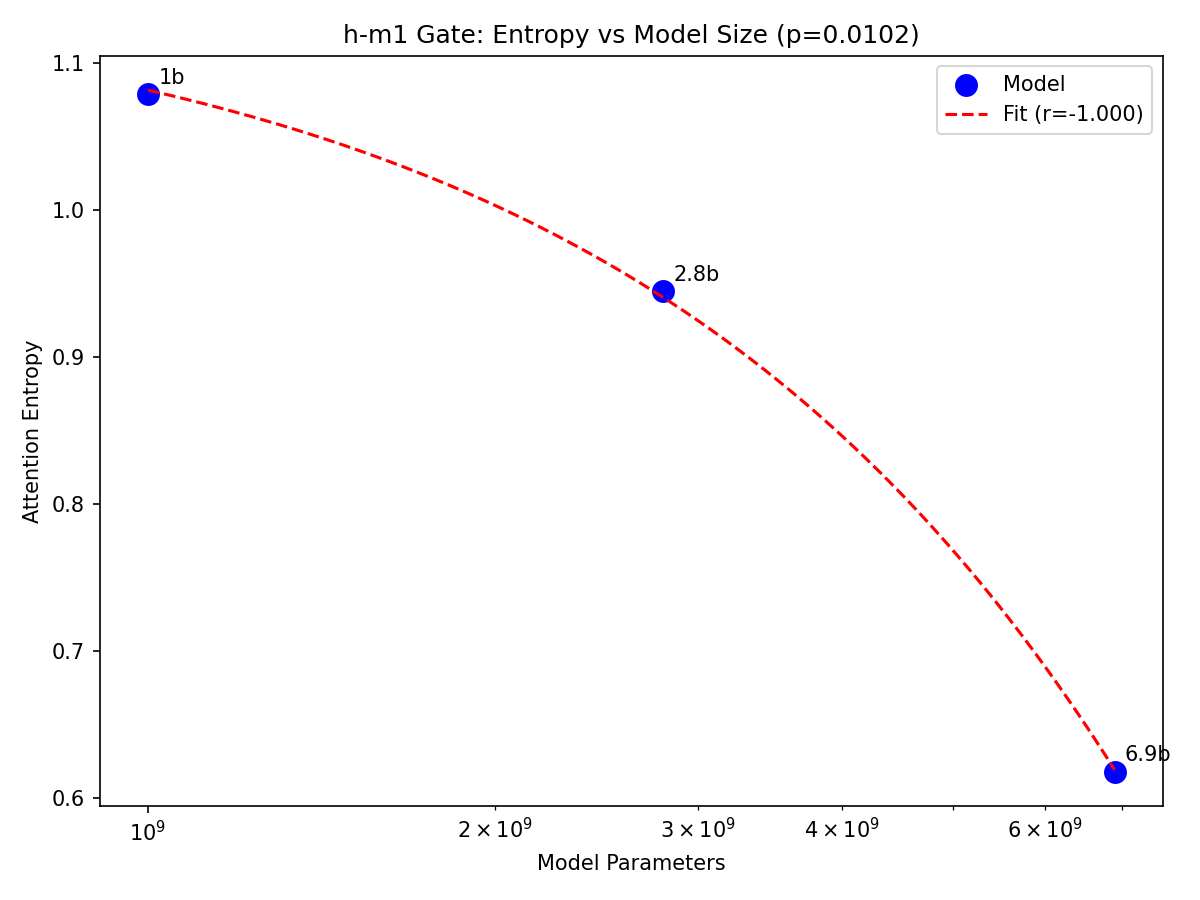
\includegraphics[width=0.8\columnwidth]{figures/fig_1_entropy_correlation.png}
\caption{Attention entropy vs model size correlation (h-m1). Contrary to our hypothesis, larger models exhibit \emph{lower} attention entropy.}
\label{fig:entropy}
\end{figure}

\begin{figure}[t]
\centering
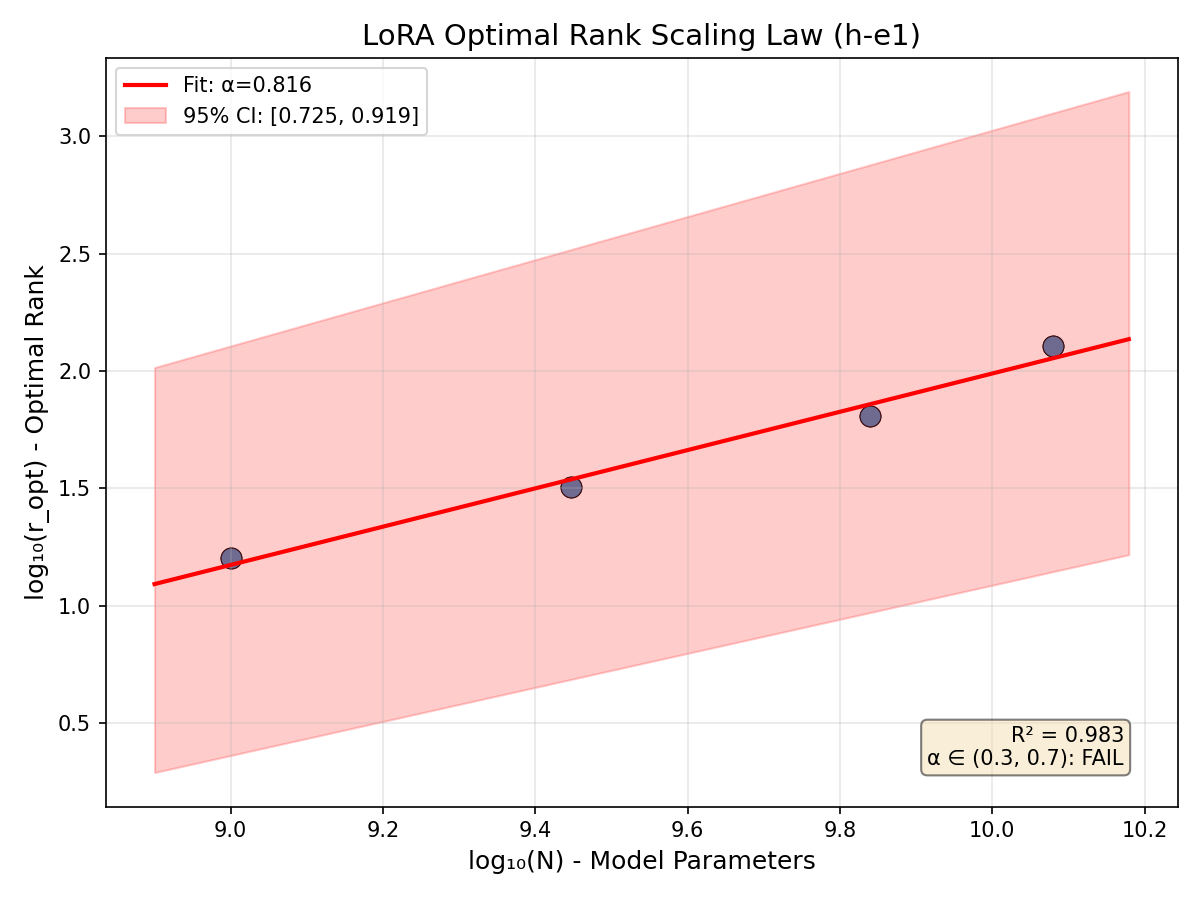
\includegraphics[width=0.8\columnwidth]{figures/fig_2_scaling_law.png}
\caption{Optimal LoRA rank scaling with model size (h-e1). The fitted power law yields $\alpha = 0.82$ with $R^2 = 0.98$.}
\label{fig:scaling}
\end{figure}

\begin{figure}[t]
\centering
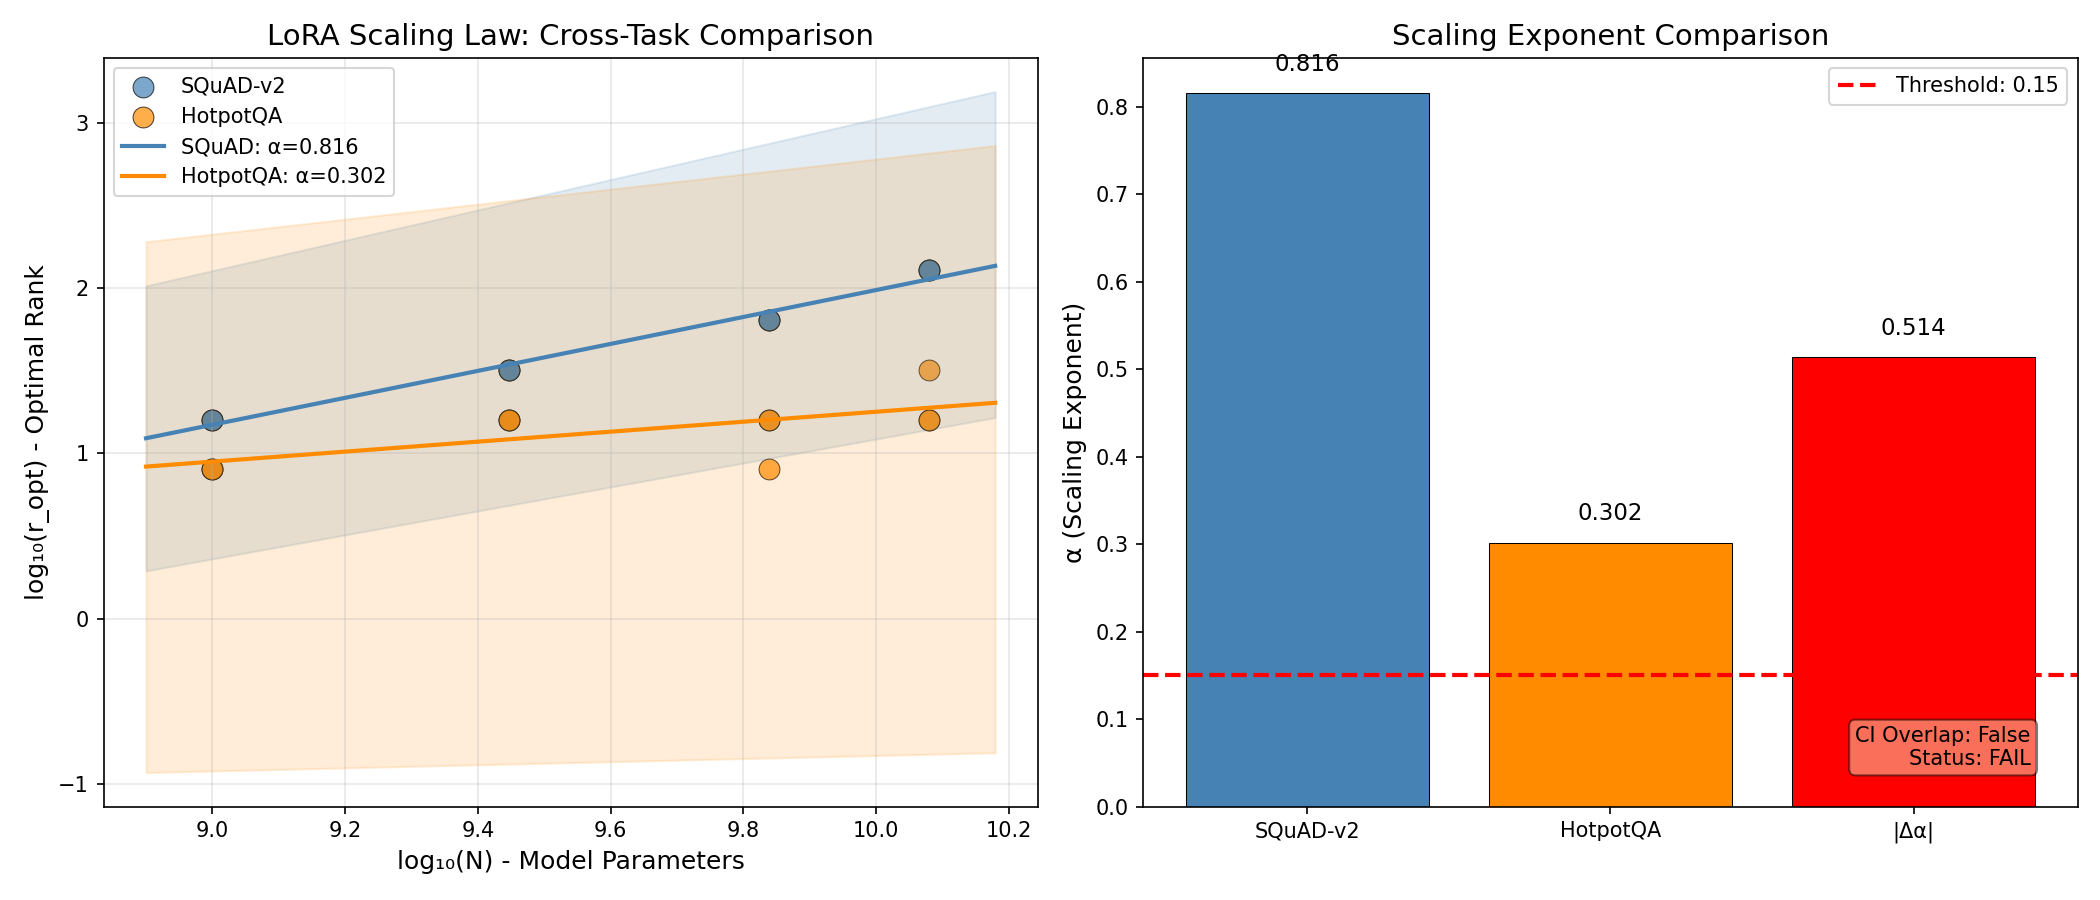
\includegraphics[width=0.8\columnwidth]{figures/fig_3_task_comparison.png}
\caption{Cross-task scaling comparison: SQuAD vs HotpotQA (h-c1). The scaling exponent differs substantially between tasks ($\alpha = 0.82$ vs $0.30$).}
\label{fig:task_comparison}
\end{figure}

\begin{figure}[t]
\centering
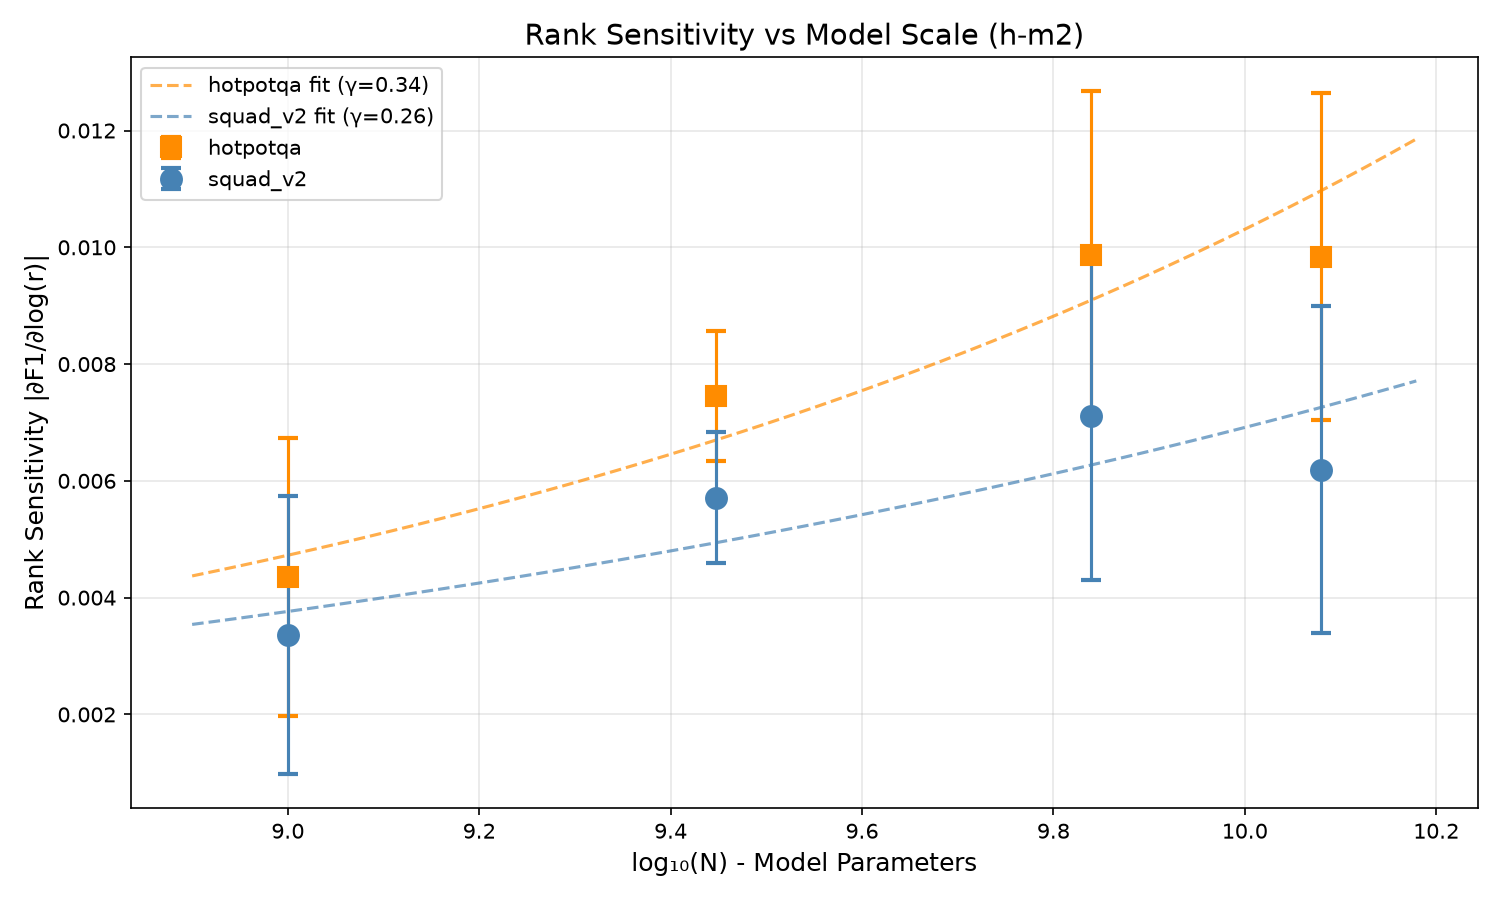
\includegraphics[width=0.8\columnwidth]{figures/fig_4_sensitivity.png}
\caption{Rank sensitivity vs model scale (h-m2). The 12B model shows 2.3$\times$ higher sensitivity than the 1B model.}
\label{fig:sensitivity}
\end{figure}

\begin{figure}[t]
\centering
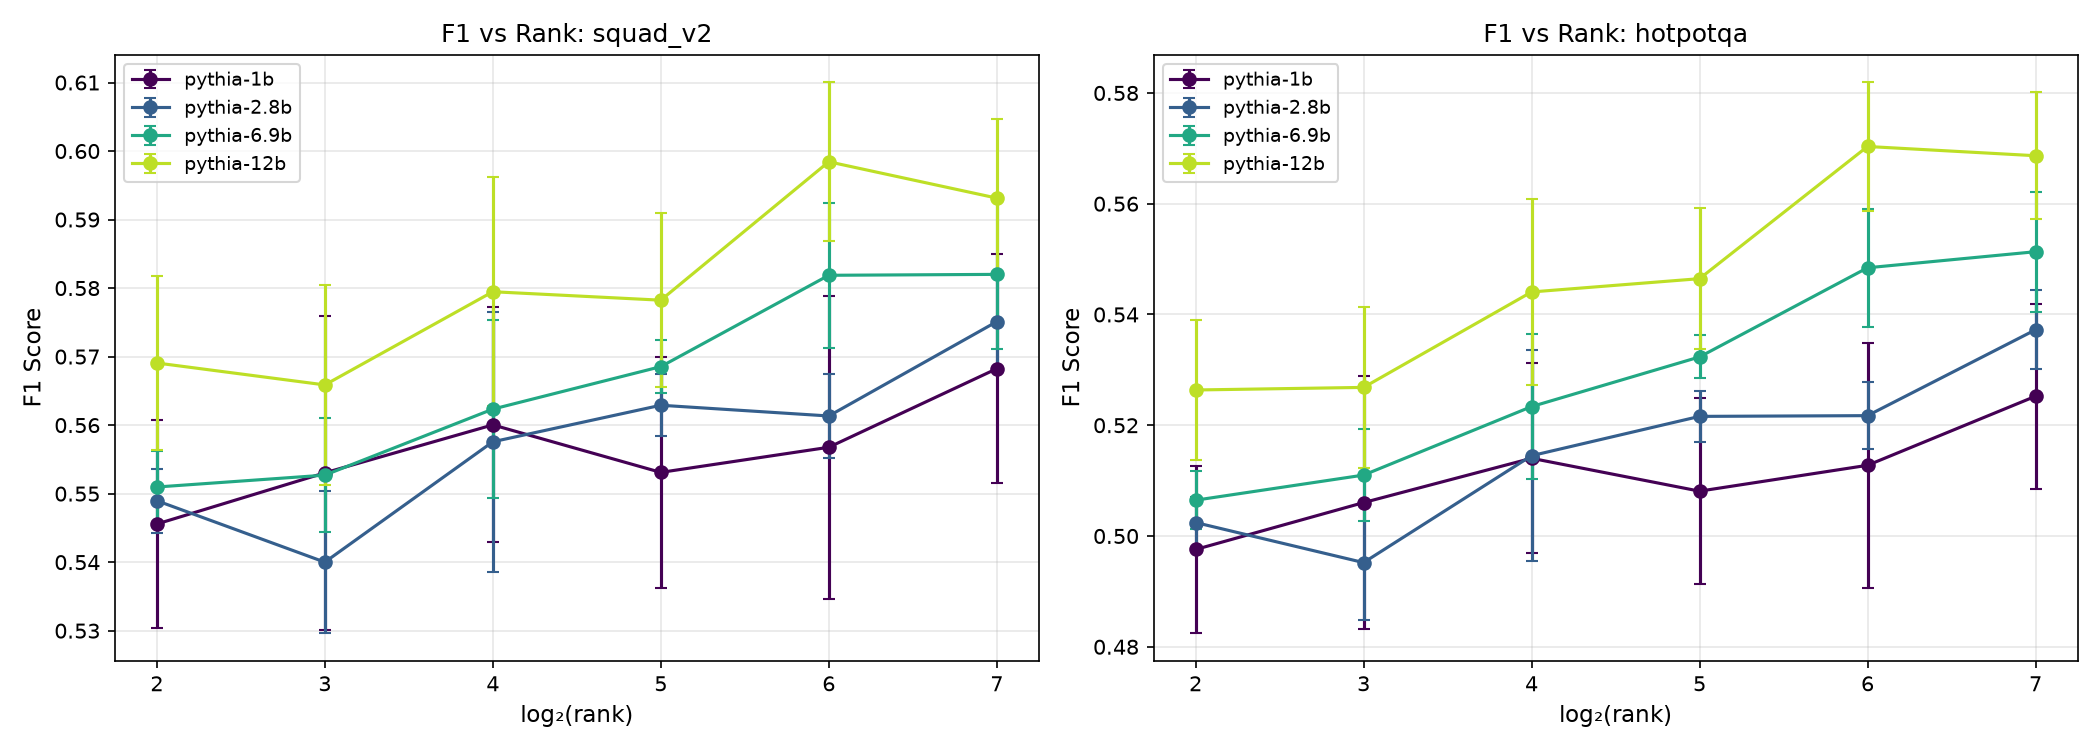
\includegraphics[width=0.8\columnwidth]{figures/fig_5_rank_curves.png}
\caption{Performance vs rank curves across model sizes (h-m2). Larger models exhibit steeper performance gradients with respect to rank.}
\label{fig:rank_curves}
\end{figure}
